\pagebreak
\subsection{Motor Friction} %\label{put a label here and uncomment}
\textbf{Name: Group 510}\\
\textbf{Date: 30/09 - 2015}

\subsubsection{Purpose}
The purpose of the test is to find the motor friction $B$ by measuring the motor current and the corresponding velocities, in several steady states.

\textbf{We extract the data from the test \textit{Generator Constant}, and so the equipment and setup is the same.}

\subsubsection{Results}
%
\begin{table}[H]
\begin{tabular}{|l|l|l| l|l|}
\cline{1-2}\cline{4-5}%-------------------------             -------------------------------------------------
  \textbf{Input (A)}   & \textbf{Output (RPM)} &\phantom{hey}& \textbf{Input (A)}   & \textbf{Output (RPM)} \\
\cline{1-2}\cline{4-5}%-------------------------             -------------------------------------------------
  $1.7$                &             $3684$    &             & $4.1$                & $21966$               \\
\cline{1-2}\cline{4-5}%-------------------------             -------------------------------------------------
  $2.2$                &             $8063$    &             & $4.8$                & $26420$               \\
\cline{1-2}\cline{4-5}%-------------------------             -------------------------------------------------
  $2.6$                &             $12021$   &             & $5.6$                & $31447$               \\
\cline{1-2}\cline{4-5}%-------------------------             -------------------------------------------------
  $3.3$                &             $16746$  \\
\cline{1-2}%------------------------------------
\end{tabular}
\end{table}
%
\begin{figure}[H]
  \centering
 	%Trim margins @:   left        bottom       right       top
 	\adjustbox{ trim = {.15\width} {.30\height} {.15\width} {.30\height}, clip }
  {
    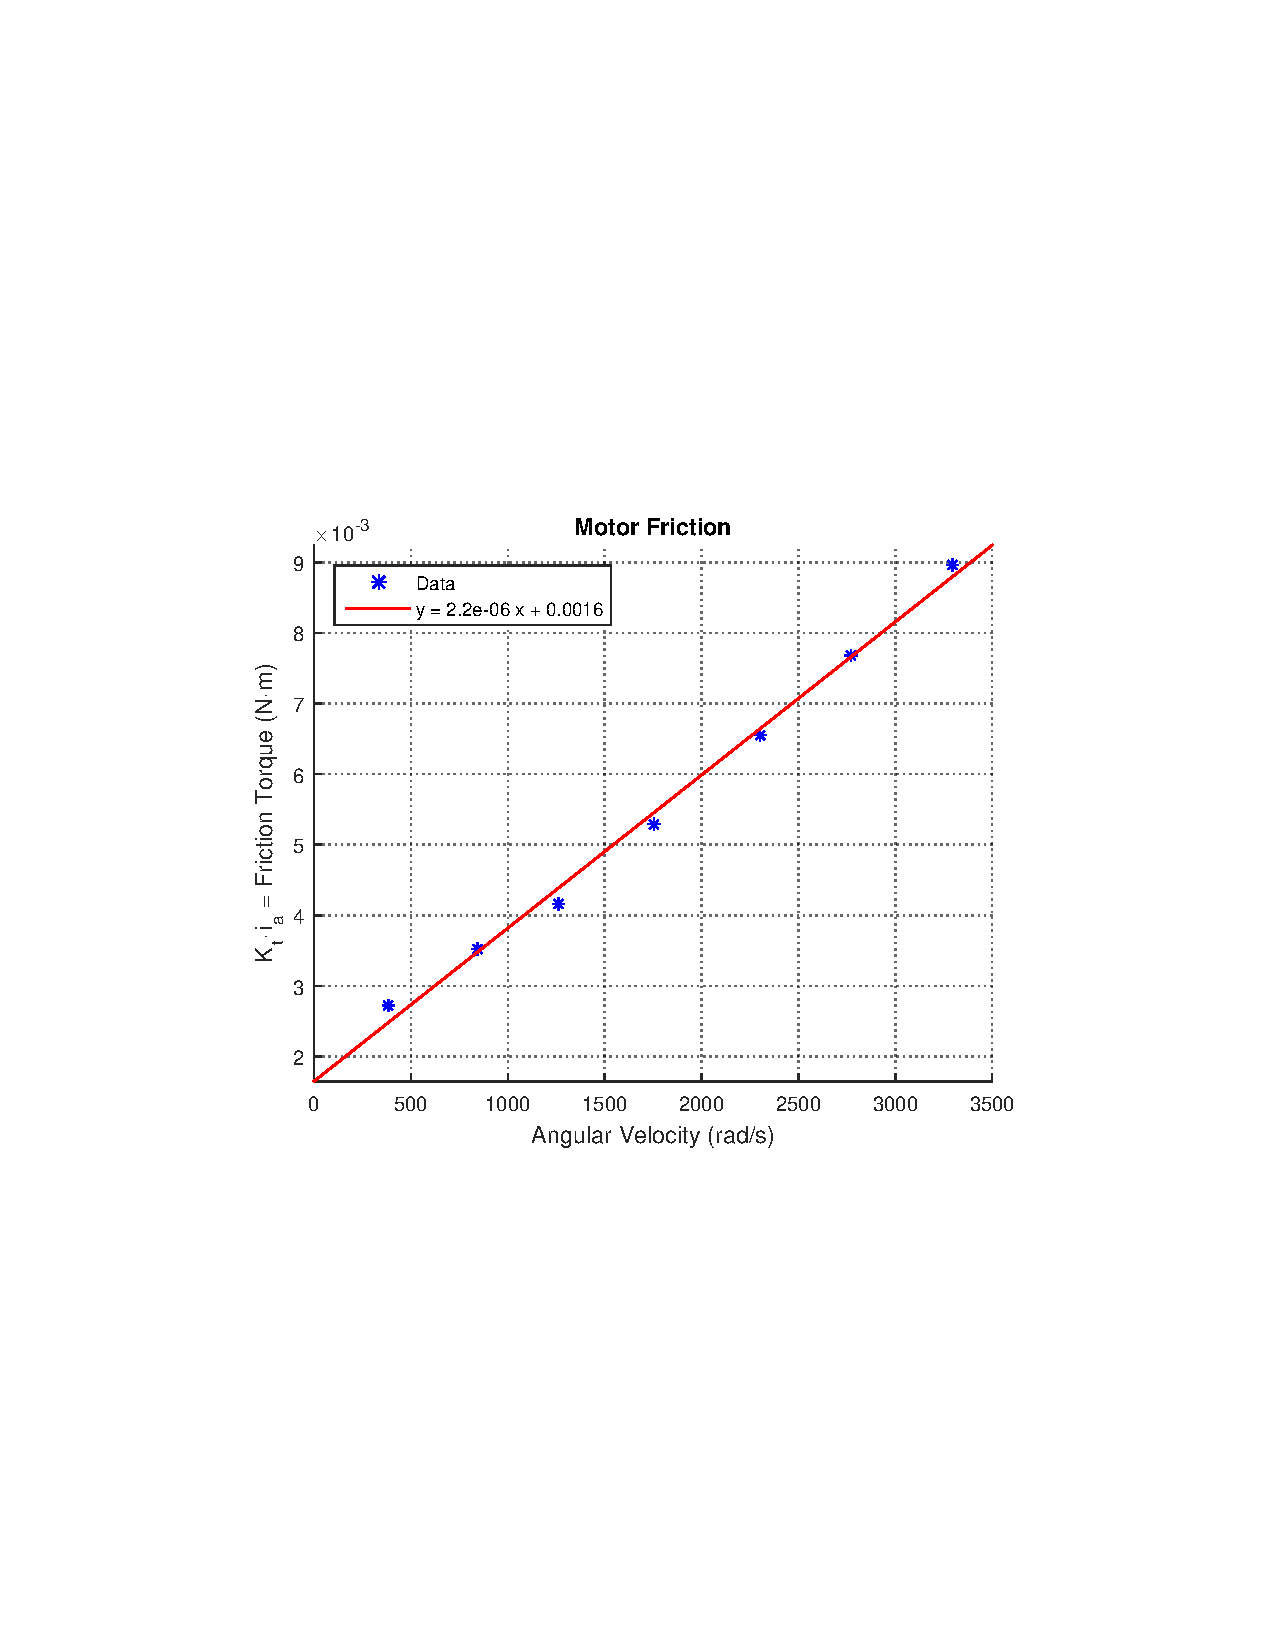
\includegraphics[width=\textwidth]{figures/motorFriction.pdf}
  }
	\caption{Plot of test results}
\end{figure}

